\begin{titlepage}

\begin{center}
\vspace*{\fill}

\Huge Reverse Engineering \RU{для начинающих}\EN{for Beginners}

\bigskip
\bigskip

\begin{figure}[H]
\centering
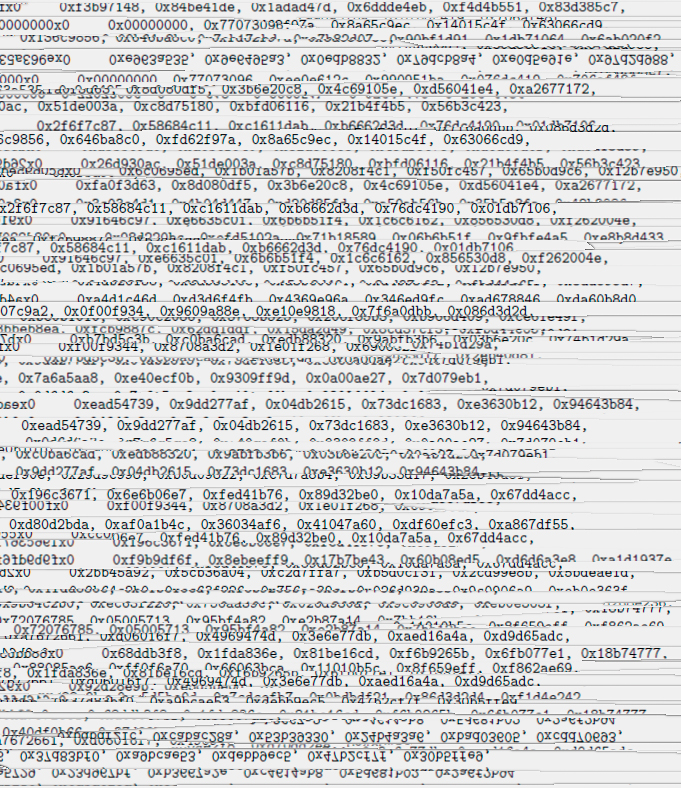
\includegraphics[scale=\FigScale]{cover.jpg}
\end{figure}

\bigskip

\hfill \huge \AUTHOR

\vspace*{\fill}
\end{center}

\end{titlepage}

\newpage

\begin{center}
\vspace*{\fill}
{\LARGE \TITLE}

\vspace*{\fill}

{\large \AUTHOR}

{\large \TT{<\EMAIL>}}
\vspace*{\fill}
\vfill

\ccbysa

\textcopyright 2013-2016, \AUTHOR. 

Это произведение доступно по лицензии Creative Commons «Attribution-ShareAlike 4.0 International» (CC BY-SA 4.0).
Чтобы увидеть копию этой лицензии, посетите \url{https://creativecommons.org/licenses/by-sa/4.0/}.

Версия этого текста ({\large \today}).

Самая новая версия текста (а также англоязычная версия) доступна на сайте \href{http://go.yurichev.com/17009}{beginners.re}.
\ifdefined\ebook
Версия формата A4 доступна там же.
\else
Версия для электронных читалок так же доступна на сайте.
\fi

Вы также можете подписаться на мой twitter для получения информации о новых версиях этого текста:
\TT{@yurichev}\footnote{\href{http://go.yurichev.com/17021}{twitter.com/yurichev}},
либо Facebook\footnote{\url{https://www.facebook.com/dennis.yurichev.5}},
либо подписаться на список рассылки
\footnote{\href{http://go.yurichev.com/17020}{yurichev.com}}.

Обложка нарисована Андреем Нечаевским: \href{http://go.yurichev.com/17023}{facebook}.

\end{center}
